\subsubsection{Om navn}
Klokken 24:00 lander jeg på den lille øya i det kalde nord. Mot
Tv-værets oppfatning befinner den seg altså ikke rett vest for
Lofoten.
Kjært barn har mange navn som man sier. Og det er gøy med navn,  så
hold dere fast! Først ble stedet funnet på slutten av 1500 tallet av
en Nederlender. Han skrev om en spiss fjellrekke i nordvest som han
følgende kalte Spitsbergen. I ettertid var ikke det god
kok for oss nordmenn. Med iherdig innsats og runetolkning av gamle
``bøker'' oppdaget vi at vikingene hadde oppdaget en øy ca. 4 dagers
seilas nord-aust for Island lenge før noen andre! Viktig å være først
si. Denne var de lite interessert i ettersom
det var verken gull eller damer her. Noe som forøvrig stemmer enda.
Neida\ldots joda\ldots telles lubne med små unger? 
Dette arktiske landskapet valgte de å kalde Svalbard. Dette kan
oversettes til Kald kyst. Eller så kan det oversettes til annet. For å
presisere sier
nordmenn Spitsbergen når vi snakker om den sør-vestlige øya med både
Longyerbyen og Barentsburg med mer (men ikke så mye). Når vi sier
Svalbard tenker vi på hele øygruppen inkludert Spitsbergen. Briter og
Nederlendere sier bare Spitsbergen og det er usikkert hva de mener.

\subsubsection*{Om klær}

For å ta det første først. Å kle seg på Svalbard er en kunst. Og den må ikke forveksles med å kle seg
i Norge. Den fella gikk jeg i. 15 blå på norsk høyfjell er ikke 15 blå
på Svalbard. I Norge kler man  seg for å gå, men på
Svalbard må man kle seg for å stå. Stå i 80kmt motvind. Det er kaldt
det. Når man går i fjellet og gradestokken begynner å trekke
ned mot 10 kalde er det helt fint med en netting, skibukse en ultrøye
og en vintett jakke. Gjerne med en god varm ullgenser i sekken som man
hiver på når appelsinen og kvikklunsjen inntas. På Svalbard må du
doble alt. Minst. Her er en liste over minstekravet for en scootertur
der alt over 60 gjør vondt.:

\begin{itemize}
		\item stilongs x3
		\item vintett skibukse
		\item to par ullsokker
		\item Fotposer (ikke tenk på at fjellsko er godt nok)
		\item ulltrøyer x3
		\item ullkofte type tykk
		\item vintett allværsjakke
		\item Tykkere jakke. Helst boble. Bomull i nød.
		\item Assecoir: polvotter, lue, buff etc etc.
\end{itemize}

Evenetuelt kan du bruke en:

\begin{itemize}
		\item Snøscooterdress
\end{itemize}

Ikke vær gnien. Lei en dress. \\

\section*{Svalbard on a shoestring}

\begin{figure}[H]
	\centering
	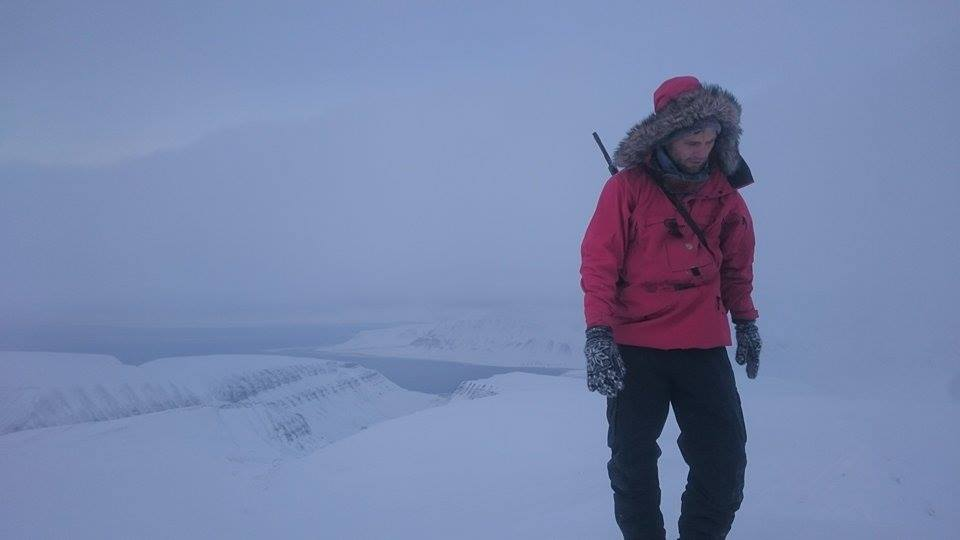
\includegraphics[width=\textwidth]{tokdubildet}
	\caption{Tok du bilde?}
\label{fig:tokdubilde}
\end{figure}

Å bo på Svalbard er dyrt. Heldigvis har jeg en kamerat jeg
tenkte å snylte litt sengeplass av. Den uskrevne regel på sofakræsjing
blant venner og medstudenter er rundt fem dager. Jeg og Jakob er veldig gode venner så går sikker helt fint
med 12. Neida\ldots joda \ldots  
Han har, overraskende nok, vært litt unvikende i hvordan vi fikser
boløsningen og
gitt svar som: 
\begin{dialogue}
	\item ``Jada, vi order noe\ldots''
\end{dialogue}
Og 
\begin{dialogue}
	\item ``Du kan sikkert bare slenge deg i stua\ldots''
\end{dialogue}\\
Så gleden er stor da jeg kommer frem
å ser at ikke bare får jeg en seng i min egen krok av stua, det er
redd opp i tillegg! Så nok en gang briljerer Jakob med sin
yndlingsteknikk: ``Increasing sucess på lowering expectations''.\\



\begin{wrapfigure}{L}{0.5\textwidth}
	\begin{center}
	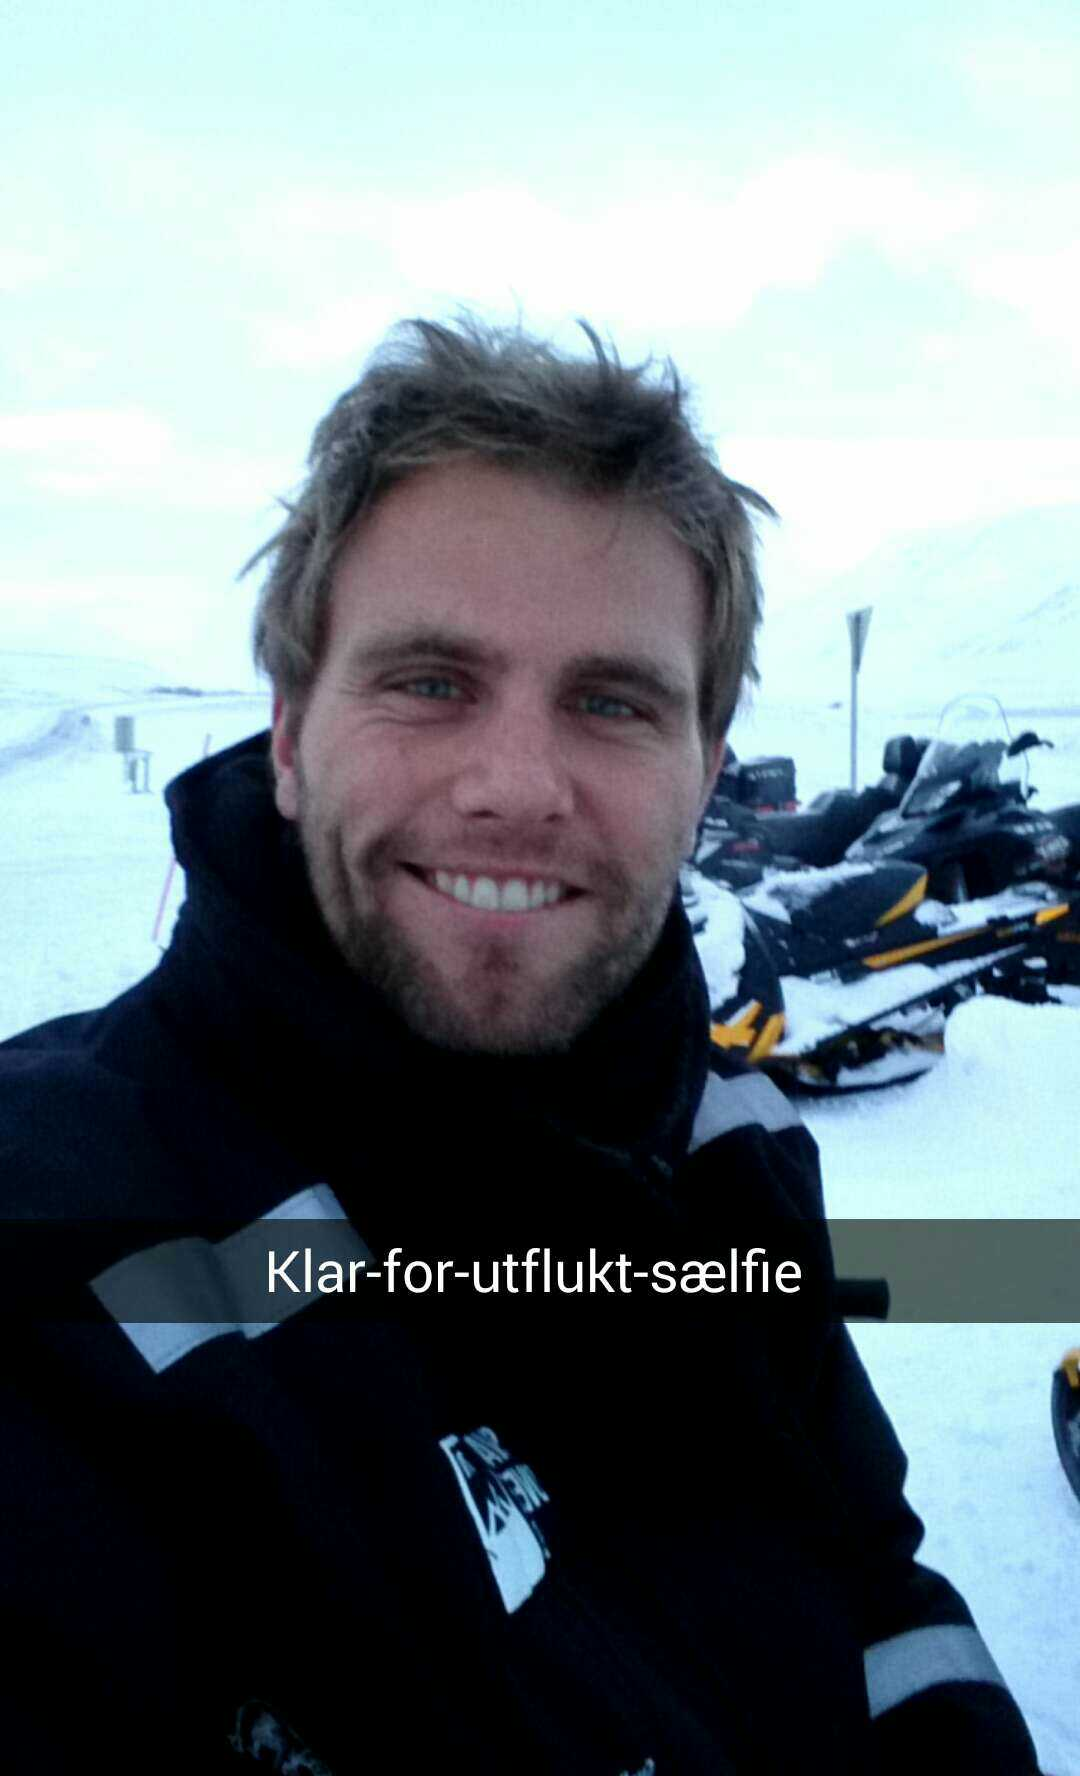
\includegraphics[width=0.48\textwidth]{klarforutsikselfie}
\end{center}
\caption{Arkisk}
\end{wrapfigure}


For tiden spilles det inn en NRK-serie på Svalbard og koppen er
kaospilot. Programmet går ut på å sette livet på spill ved å bekrefte
fysiske lover. Feks ta på seg en metalldress og bruke seg selv som en
lynavleder for å vise a at strømmen går letteste vei. Jeg bidrar på
settet som skuelysten. Å være ute blandt folk leder som regel til noe 
bra og dette var ikke et unntak. Da produksjonsgjengen leier inn Jakob for en snøscootertur til
Barentsburg blir jeg invitert. 2 timer senere har jeg lånt scooter,
dress og er klar for action. Turen var ingenting kort for fantastisk.
Den inspirerte tiraden som står under titelbilde til Svalbard kom som
følge av denne turen. Bare tro meg når jeg sier at det føles helt
annerledes enn Jotunheimen og alpene. Alt er så mye mer
``arktisk''. Fra vinden som pisker deg i ansiktet til isfjell(pengu) som
stikker opp av bakken.


\begin{figure}[!h]
	\centering
	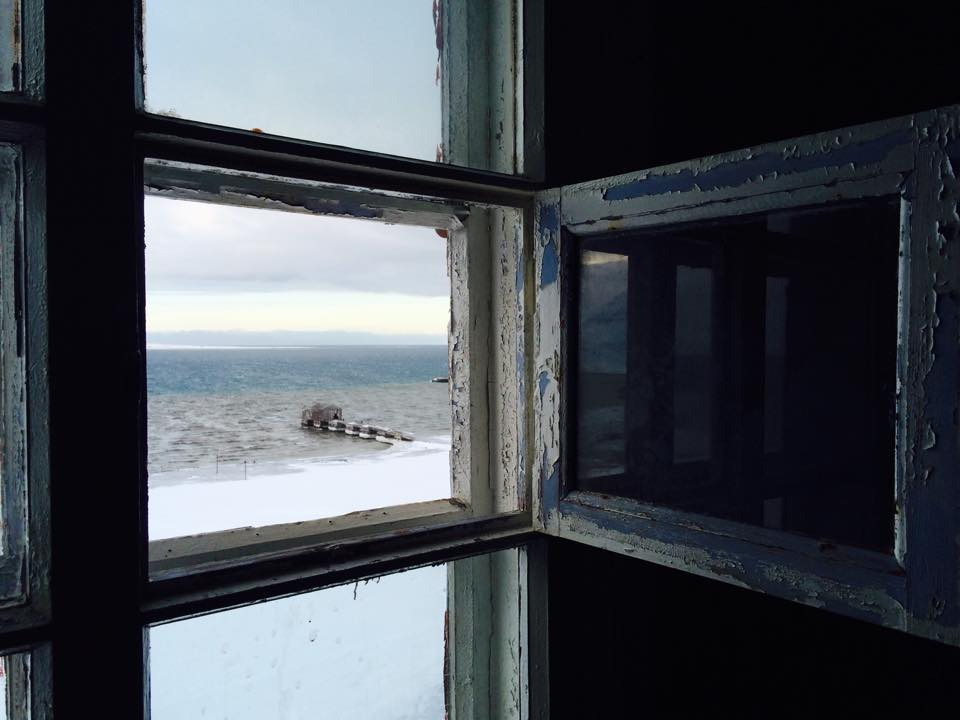
\includegraphics[width=\textwidth]{Colesbay}
	\caption{Coles bay}
\label{fig:tilbarentsburg}
\end{figure}

Vi sjekker inn etter solnedgang i Barentsburg. Jeg er selvfølgelig
guide-under-opplæring
og sover på rommet til Jakob for en billig penge. Svalbard er norsk
sier de. Ok. De har ikke vært i Barentsburg. Kråketegn istedenfor
bokstaver, fint sentrum og rønner utenfor. Guider som åpenbart driver
propaganda setter prikken over i'en. Russisk nok for meg. Tross dette var Tv-kanalene spikeren
i kista. Vi Var overbevist om at
vi så på et fiskeprogram før de etter 30 minutter prøvde å selge oss
fiskestanga. \#Verdenslengstereklame. På hjemturen dro vi innom Coles
bay. Min beste beskrivelse vil være et arktisk
Chernobyll. Dette var før en gruve og en havn for skip som skulle
 hente kull. Så dro folk. På dagen. Huset og møblene har
fått klare seg selv. Forlatt, kaldt og panoramautsikt. Klarer man ikke
beksrive det med mange ord lønner deg ofte med få! Disse husene har
ofte blitt ly for isbjørner. Så litt sibo blir det når Jakob skal
sjekke alle rom med rifla. Under er det kart over ruta vår. 

\begin{figure}[h!]
\centering
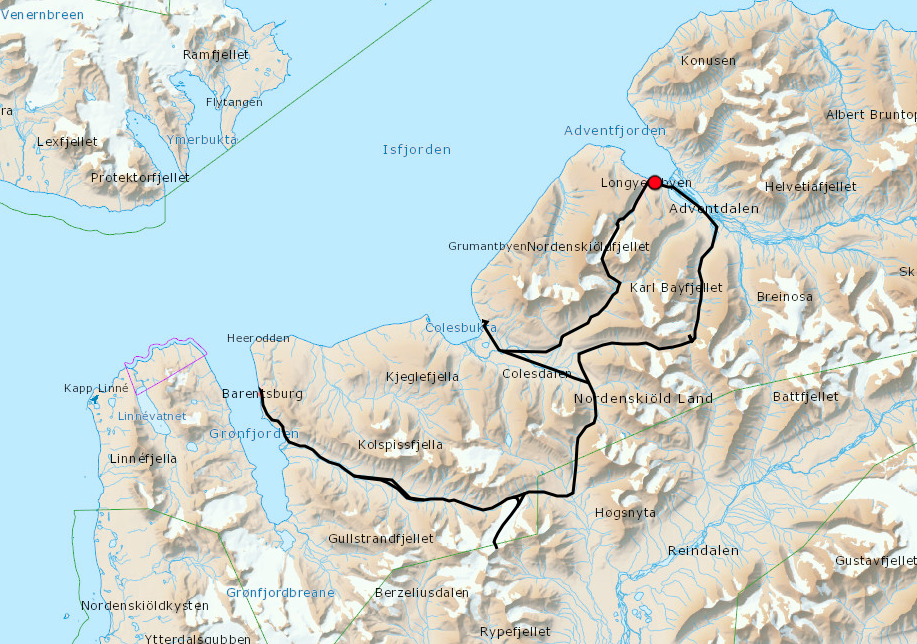
\includegraphics[scale=0.22]{Turbarentsburgliten}
\caption{Detaljert kart}
\label{fig:barentsburgturliten}
\end{figure}

\begin{figure}[h!]
\centering
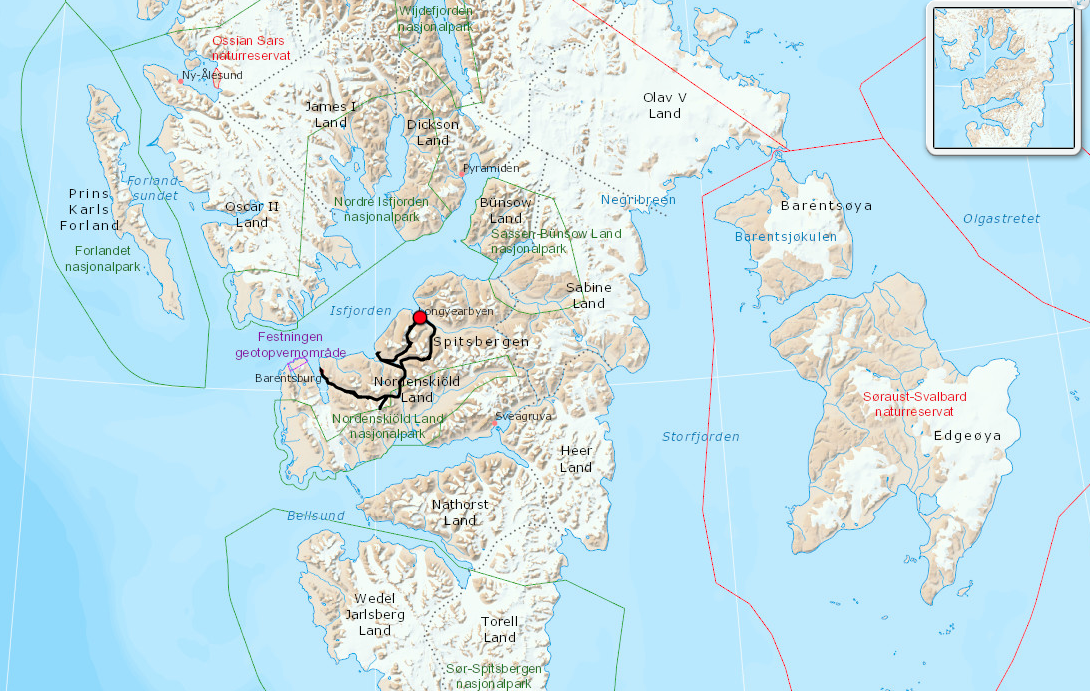
\includegraphics[scale=0.22]{Turbarentsburgstor}
\caption{Oversiktskart}
\label{fig:barentsburgoversiktskart}
\end{figure}
Hellet snur ikke enda og jeg får bli med på en guidet tur neste dag
også! Da drar vi helt inn i Tempelfjorden (sett inn bilde), ser
brefronten og spiser en særdeles god lunsj på en seilbåt som fryser
seg inn i isen (med vilje) hver vinter. På veien stopper vi også med
det mest kjente trapper-redet. Der Jakobs idol tilbrakte 38 vintere
som fangstmann. Ikke nok med det, han lurte med seg hele to damer opp
til å bo med ham (ikke på en gang). Første var ikke så keen på å være her på vinteren,
men han tok henne bare opp med siste båten! Hun endte opp med å føde
alene her på Svalbard mens han rodde til Longyerbyen for å hente
legen. Dette var visst ganske traumatisk og hun tilbrakte resten av
sine dager på psykiatrisk avdeling. Happy days. Fangstmannen fikk
heldigvis opp en ny dame. Så det ordnet seg for alle parter.\\

\begin{figure}[h!]
	\centering
\noindent\makebox[\textwidth]{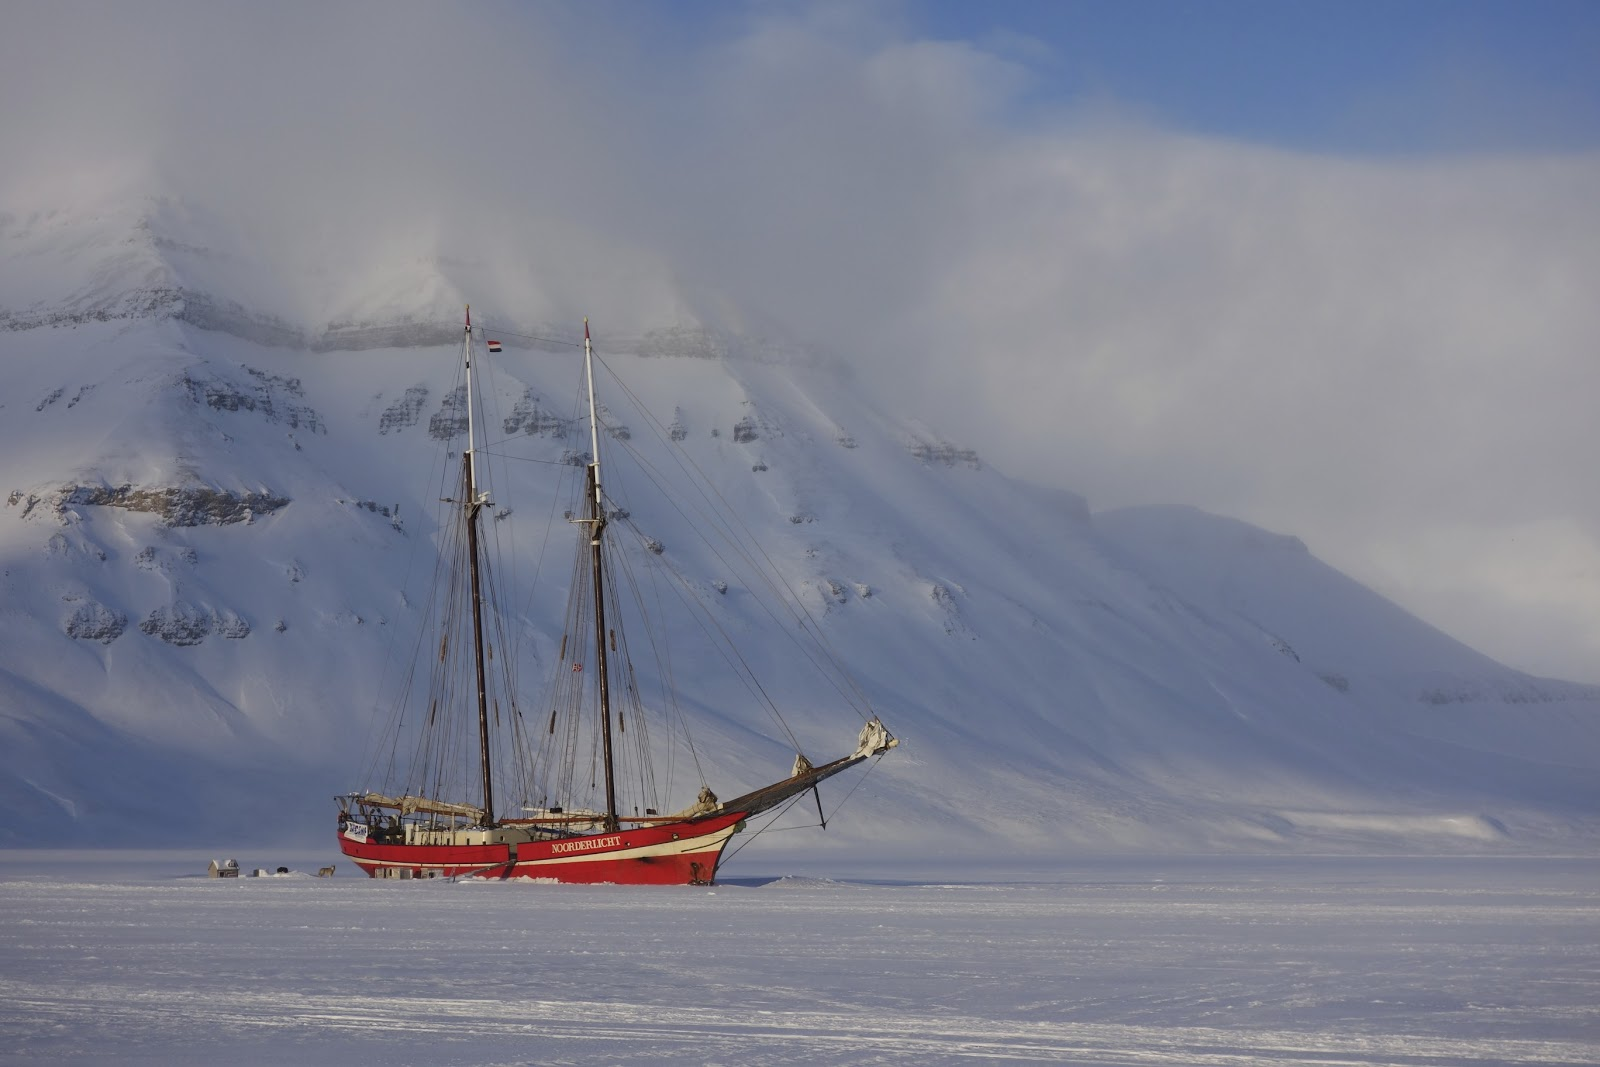
\includegraphics[width=\paperwidth]{baatis}}	
%	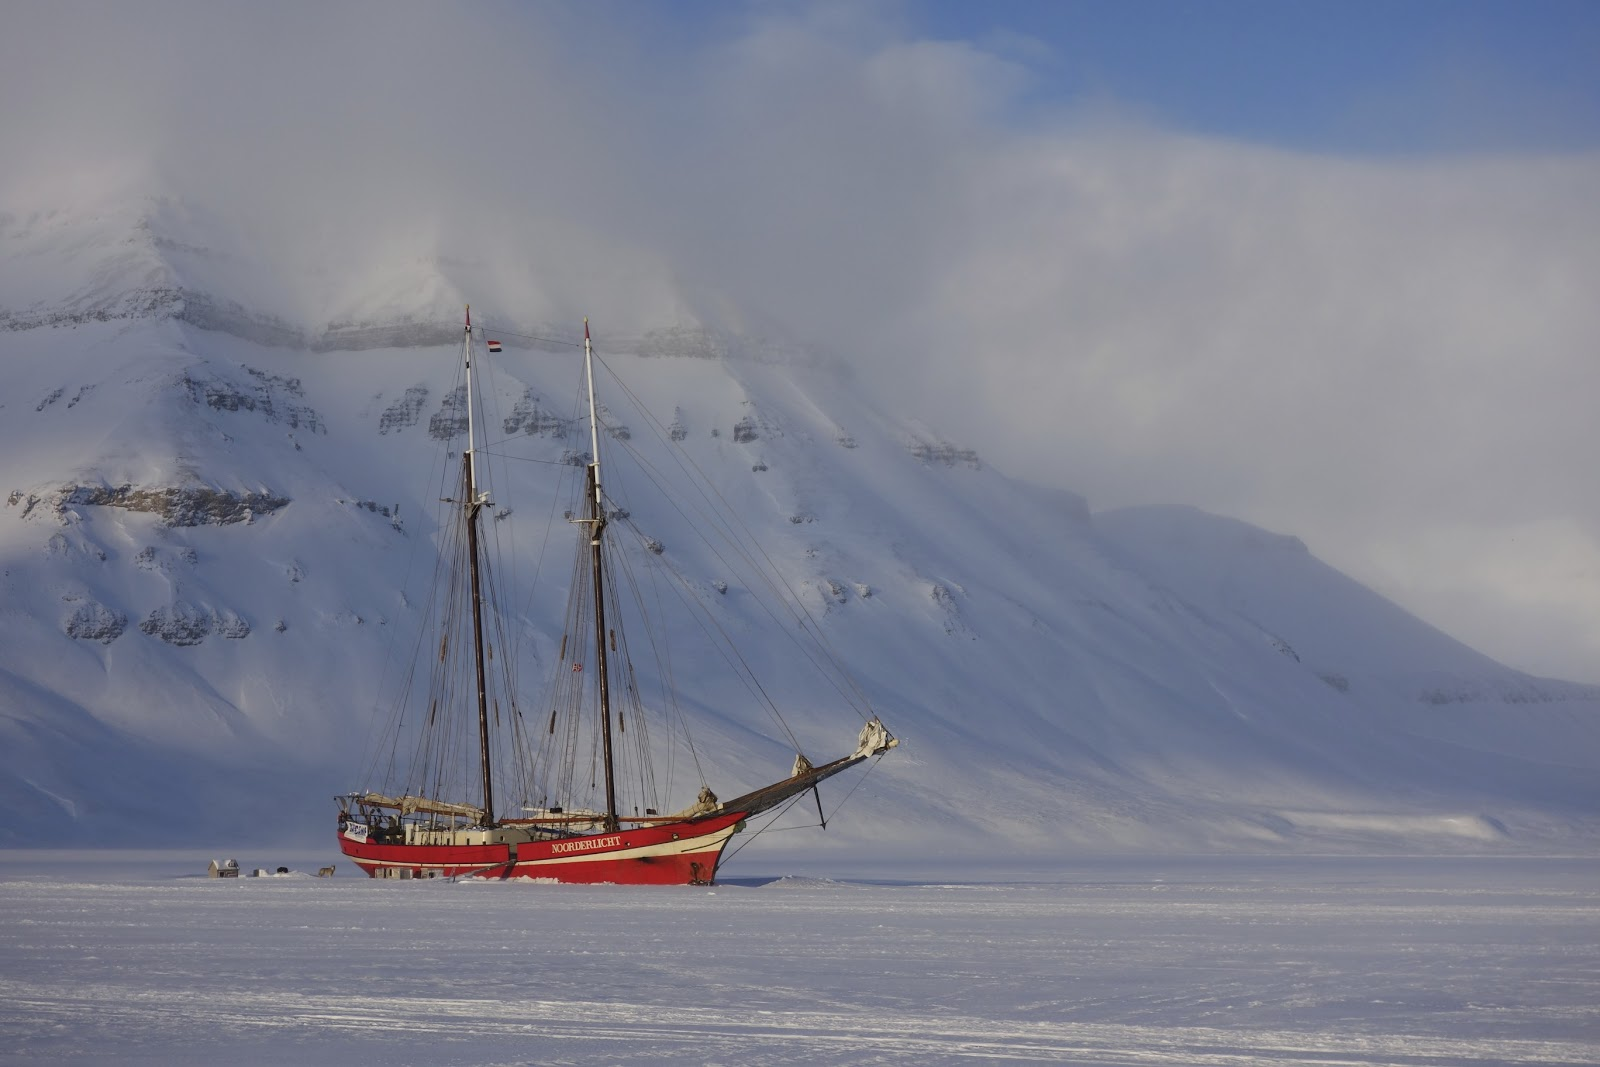
\includegraphics[height=\paperheight]{baatis}
	\caption{Båtis}
\label{fig:båtis}
\end{figure}


%\begin{figure}[!h]
%	\centering
%	\includegraphics[width=\textwidth]{trollsteinen}
%	\caption{Viktig å være på toppen}
%	\label{fig:trollteinen}
%\end{figure}
Gullhåret fortsetter å gro i rumpa og neste dag får jeg bli med på
hundespann! Kjæresten til Jakob er nemlig hundefører. Hundespann er en opplevelse fra a til å. Man begynner med å få på seg
polardressen. Deretter går man inn i hundegården. Det er to ting disse hundene liker:
løping
og mennesker. Og bare sistnevnte siden det ofte leder til det
førstnevnte. Når man setter foten inn i hundegården ville selv den
mest populære tenåringsjente fått
tilfredsstilt oppmerksomhetbehovet sitt. Alle hundene vil hilse på.
Samtidigt. Det blir ikke bedre når du tar frem selen til sleden.\\

Tanken med hundespann  er at det skal være mer enn en tur
med hund fra A til B der du sitter på. Du skal selv finne frem hundene, deretter
skal du sette dem fast til sleden og til slutt skal du kjøre. Du får
altså styre din egen slede. Og med styre mener jeg bremse. Fordi det
er egentlig den eneste form for styring oss dødelige har.
Guiden kan rope høyre og venstre til de ADHD-avlingene og da hender det
de svinger\ldots kanskje.

\begin{figure}[h!]
	\centering
	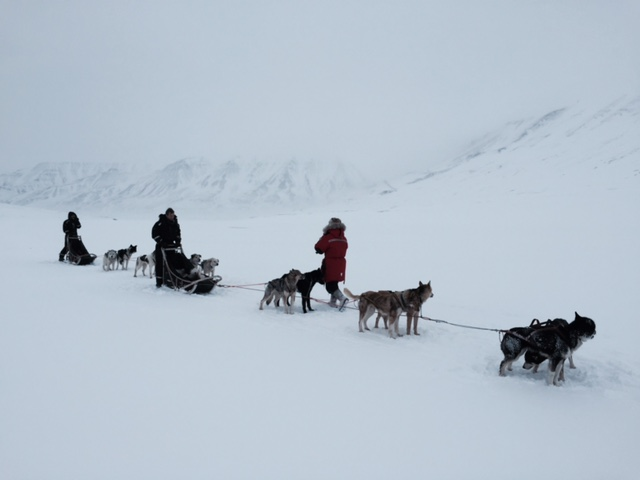
\includegraphics[width=\textwidth]{Hundespann}
	\caption{Hundespann}
\label{fig:hundespann}

\end{figure}
\begin{figure}[H]
	\centering
\noindent\makebox[\textwidth]{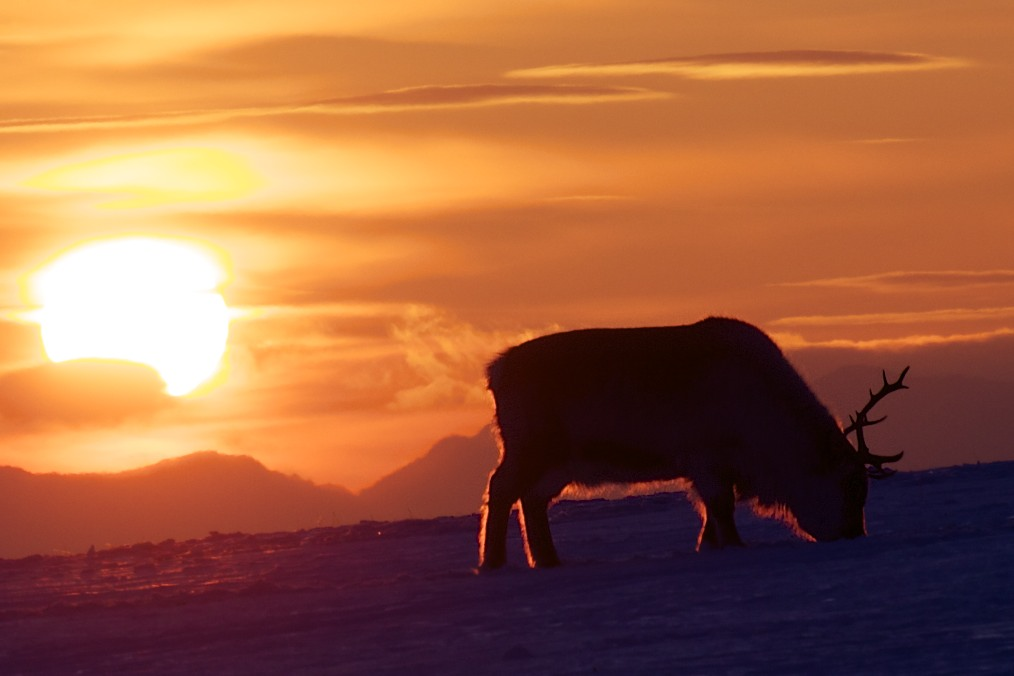
\includegraphics[width=\paperwidth]{reinisolnedgang}}	
	\caption*{Rein i Solnedgang: tatt av Stianmedsekken}
\label{fig:rein}
\end{figure}
\subsubsection{Om Svalbardrein}

Svalbardreinen er verdens nordligste planteetende pattedyr. Det er to teorier om hvordan
den kom til øya. Enten utvandret den fra Grønland over havisen under
forrige istid. Eller så vandret den seg nordover fra kontinental
Europa da klimaet ble varmere. Den har uansett vært isolert her i
tusen år og utviklet mange særtrekk for å overleve det harde klimaet.
Når du først ser et Svalbardrein vil du anta det er en kalv. Det
er sansynligvis feil ettrosm alle svalbard rein er korte\ldots og feite.
Skikkelig feite. Det er for å holde gjennom en kald vinter med lite
mat. I tillegg til kropsfasongen har de også andre hjelpemidler for å
takle kulda. Den mest interessante av disse er varmevekslere i nesa og
bena. En Svalbardrein får aldri damp på utpust. Det er fordi
luften den puster ut er nesten like kald som omvigelsestemperaturen.
Den får til dette med å ha en varmeveksler i nesa som varmer opp lufta
som skal inn ved å kjøle ned lufta som skal ut. Ganske fantastisk.\\

Blodet til et menneske
er ca 37grader i hele kroppen. En Svalbardrein kan imidlertid ha
blodet helt ned til 8grader i bena. Dette er for å minske varmetapet
til bakken. Blodårene går så i en spiral opp til hjertet igjen for å
varme blodet før det går inn. Selv en Svalbardrein ville dødd om blodet
som går inn i hjertet holder 8grader. \\

De går svært sjeldent i flokk. Det er to grunner til dette. For det
første har de ingen naturlige fiender. Isbjørnen er en sprinter mens
reinsdyr er maratonløpere. Den skal være veldig heldig om den får
fanget en. For det andre er det så lite med mat på Svalbard at om de
beitet sammen ville det ikke vært nok. Det som er vittig er at de ikke
blir eldre enn 10 år. De spise nemlig alt de kommer over på vinteren.
Følgende spiser de mye grus. Dette sliper gradvis ned tennene. Så
etter ca. 10 år dør de endten av blodforgiftning eller sult. Sa jeg
vittig? Jeg mente tragisk. Men som de sier: ``Humor er tragedie pluss
tid.`` Du får prøve å lese det igjen om et par år å se om du humrer
litt da!\\

Det er jakt en gang i året på reinen for å kontrollere befolkningen.
Med jakt mener jeg henrettelse. Reinsdyret har nemlig ikke rukket å
bli redd mennesker enda. Så man går bort, klapper det litt, skyter det
og går hjem. Alt før lunsj. Vittig.





\subsection*{Fiffen feirer best}

Etter å ha hengt med representanter Cavacorner i Rio skulle man trodd
det ble et kulturkræsj å slå seg ned hos freelance karene i vei 226 A
Svalbard. Det var både ja og nei. Cava ble det bare mer av! På
Svalbard er det nemlig kvote på øl og sprit. Dette er av
tradisjonsgrunner ettersom det var det gruvearbeiderne drakk. Vin og
bobbler var det eierne og direktørene som drakk derimot. Så det er det
fri flyt av! Følgende var det ikke svette karer og øl da Jakob feiret
bursdagen.Det var svette karer og Cava. God stemning. Som offergave
til leiligheten kjøpte jeg inn 4 flasker sprudlemoro og tok det
derfra!\\


Etter dette gikk dagene litt i ett. Jakob var mye opptatt med jobb, og
jeg satt pris på litt alenetid. Var nesten 3 måneder siden jeg hadde
vært alene. På kveldstid fant vi selvfølgelig på noen sprell. Tau og
ski etter snøscooter er jo en match-made-in-heaven. Problemet er at
det ligner litt for mye på vannski, men det har noen vesentlig
forskjeller. Viktigst av disse er at det  ikke er like
artig å falle. Noe man fort kan glemme når man er i siget. Følgende
hang jeg etter i godt over 80 da vi dundret forbi en
barnehageklasse som var på tur. Viktig å se at vi enda ikke er for
gamle til å fremprovosere noen hakeslepp på barnehagetanter.\\
\begin{figure}[]
	\centering
	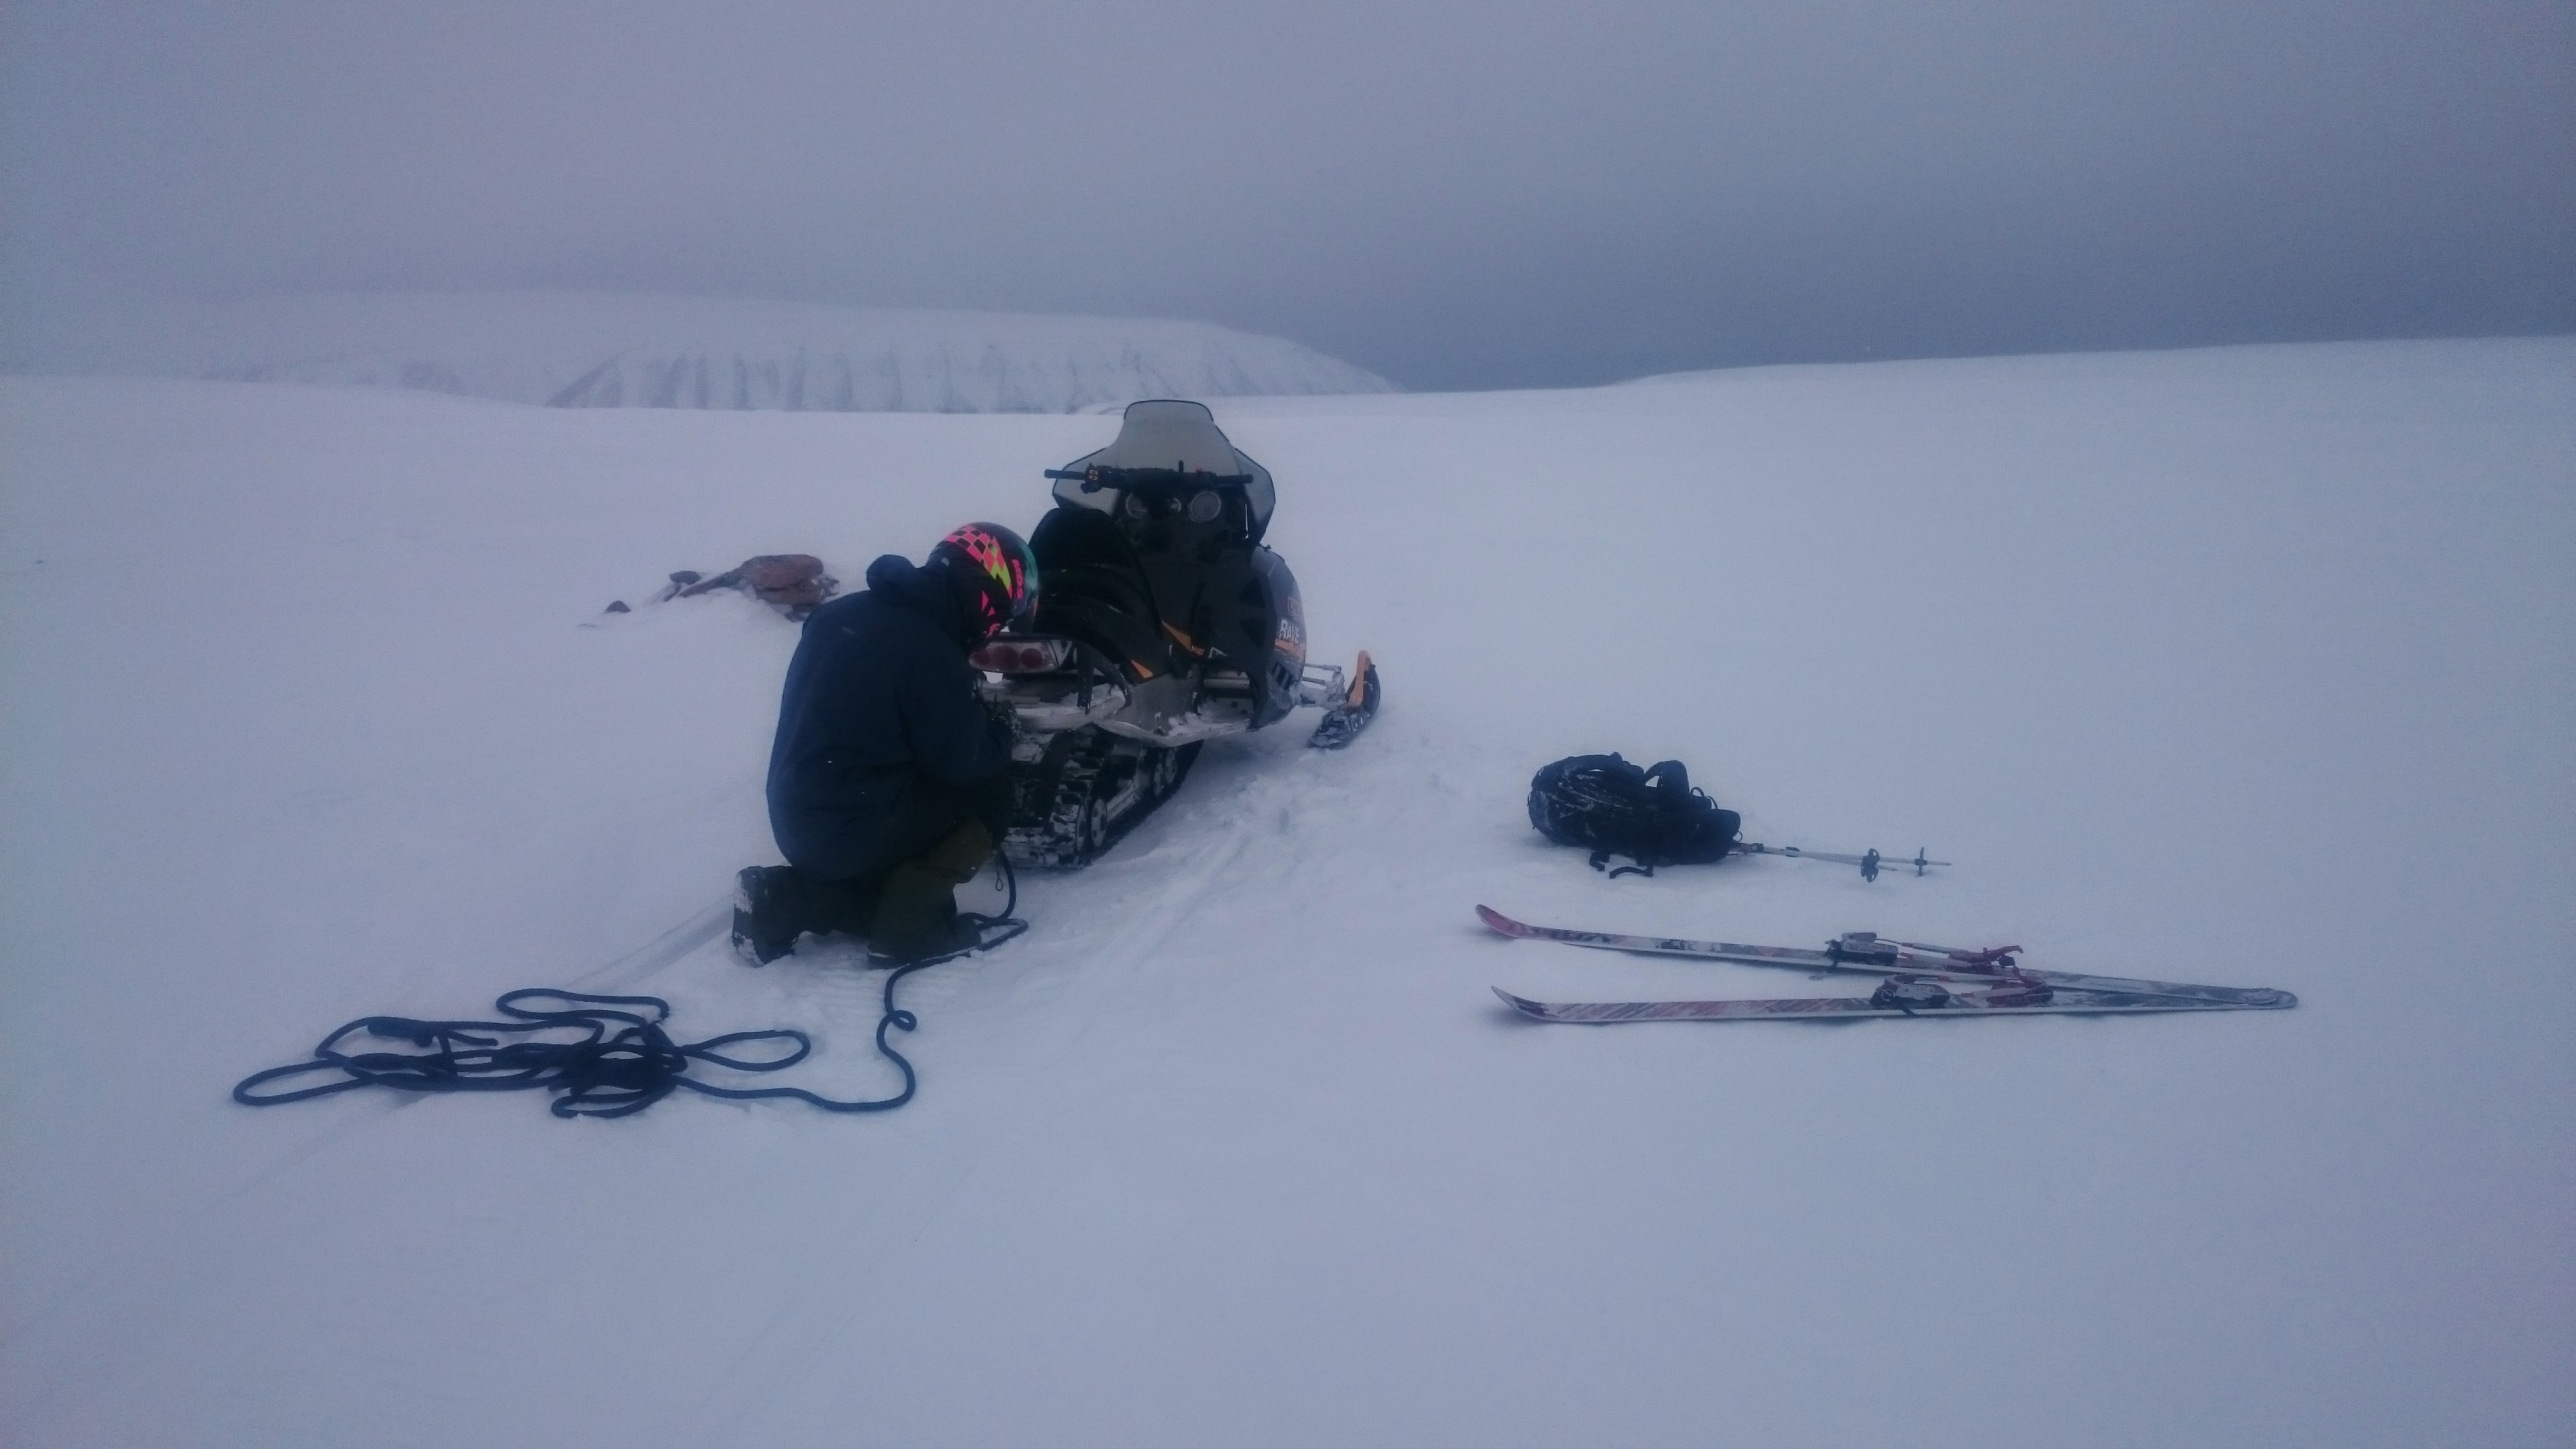
\includegraphics[width=\textwidth]{Scooterogski}
	\caption{Suksessoppskrift}
\label{fig:trollsteinen}
\end{figure}

Etter
ble jeg forkjølet. Noe som egentlig bare var et problem da jeg ikke
hadde det gøy. Så veldig syk var jeg ikke. Vi fikk spent på oss skiene
tatt en tur opp til Trollstien og kjørt snøscooter
i Fardalen i sola. Avslutter elegant med å  hjelpe noen gale spanjoler
fly luftballong. 8 velt hadde de med snøscooteren på veien tilbake. Må
være rekord. Scooter er som å sykle, går det for sent velter man. Er
imidlertid vanskelig å sette tempo når man da konstant får høre
bakfra fra Conzuela
\begin{dialogue}
	\item ``Jakob no espeedo'
	\item ``no espeedo Jakob'
	\item ``Jakob no no'
\end{dialogue}
\\
Bilde fra luftballong
(bilde fra trollstien)

%hva er nok tøy? annerledes å stå stille. tre stilongs. netting løsere
%devold. strammere devold. ullgenser tykk. vinnjakke goretex. bomull. 

